\documentclass{ximera}
\graphicspath{ {./images/} }

\begin{document}
\section*{Catalog Description:}
Algebraic, rational, and radical expressions; functions and graphs; quadratic equations; absolute value; inequalities; and applications.

\section*{Prerequisite:}
Math Placement Level S, a grade of C- or better in Math 1050, or credit for Math 75 or 1074.

\section*{Exclusions:}
Not open to students with credit for any higher numbered math class, or for any quarter math class numbered higher than 75.

\section*{Text:}
Beginning and Intermediate Algebra ( $4^{\text {th }}$ ed), OSU Custom version, Miller, O'Neill \& Hyde, McGraw-Hill, ISBN 9781259541650

\section*{Follow-up Courses:}
\begin{itemize}
  \item Math 1116 for students in liberal arts or students in the precertification programs on regional campuses.
  \item Math 1125 for students intending to pursue a M.Ed. in early or middle childhood.
  \item Math 1130 College Algebra for Business
  \item Math 1148 Traditional College Algebra
\end{itemize}

\section*{Sequencing Chart:}
%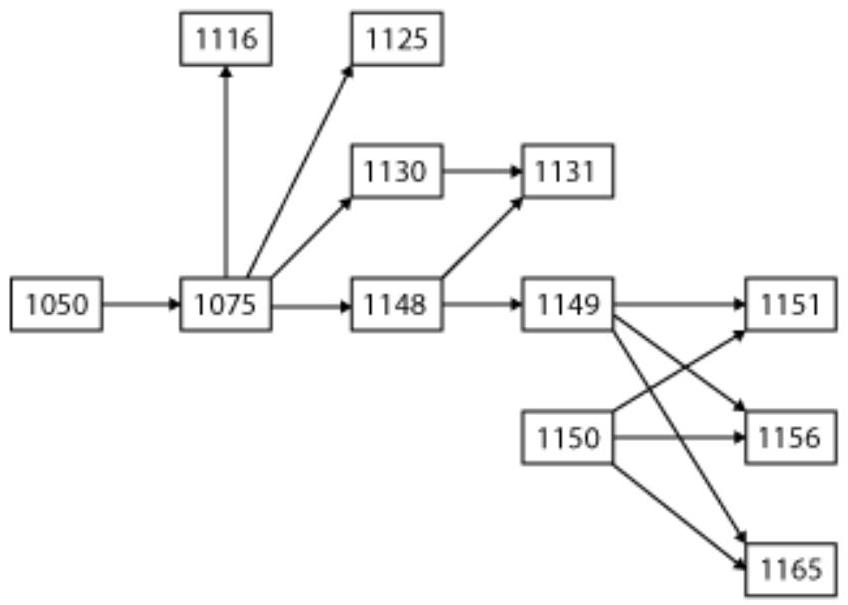
\includegraphics[alt={Flowchart showing Math course sequencing from 1050 through 1075 to upper-level courses including 1116, 1125, 1130, 1148, 1149, 1150, 1151, 1156, and 1165},width=\textwidth]{course-sequencing-chart}\\
Topics List:\\
Ch. 4 Linear Inequalities\\
4.1 Solving linear inequalities using addition \& subtraction\\
4.2 Solving linear inequalities using multiplication \& division\\
4.3 Solving compound inequalities\\
4.4 Solving absolute value equations \& inequalities\\
4.5 Graphing systems of inequalities in two variables\\
Ch. 6 Factoring Polynomials\\
6.1 Introduction to factoring polynomials\\
6.2 Factoring trinomials of the form $x^{2}+b x+c$\\
6.3 Factoring trinomials of the form $a x^{2}+b x+c$\\
6.4 Factoring special binomials\\
6.5 Factoring by grouping; General strategies for factoring\\
6.6 Solving equations by factoring\\
Ch. 9 Rational Functions\\
9.1 Graphs of rational functions\\
9.2 Reducing rational expressions; Multiplying and dividing rational expressions\\
9.3 Adding and subtracting rational expressions\\
9.4 Combining operations; Complex rational expressions\\
9.5 Solving equations containing rational expressions\\
9.6 Inverse and joint variation; Other applications yielding equations with fractions\\
Ch. 7 Solving Quadratic Equations\\
7.1 Extraction of roots and properties of square roots\\
7.2 Solving quadratic equations by completing the square\\
7.3 The quadratic formula\\
7.4 Applications of quadratic equations\\
7.5 Complex numbers; Solving quadratic equations with complex solutions\\
Ch. 8 Functions: Linear, Absolute Value, and Quadratic\\
8.1 Functions and representations of functions\\
8.2 Linear Functions\\
8.3 Absolute value functions\\
8.4 Quadratic functions\\
Ch. 10 Square Root \& Cube Root Functions and Rational Exponents\\
10.1 Evaluating radical expressions\\
10.2 Adding \& subtracting radical expressions\\
10.3 Multiplying \& dividing radical expressions\\
10.4 Solving equations containing radical expressions\\
10.5 Rational exponents \& radicals


\end{document}